% LaTeX source for ``Algorithms for Computer Simulation of Molecular Systems''
% Copyright (c) 2023 รังสิมันต์ เกษแก้ว (Rangsiman Ketkaew).

% License: Creative Commons Attribution-NonCommercial-NoDerivatives 4.0 International (CC BY-NC-ND 4.0)
% https://creativecommons.org/licenses/by-nc-nd/4.0/

\chapter{พลวัตเชิงโมเลกุลแบบดั้งเดิม}
\label{ch:aimd}

%----------------------------------------
\section{การจำลองเชิงตัวเลขและเทคนิคเชิงคอมพิวเตอร์}
%----------------------------------------

การจำลองเชิงตัวเลข (Numerical Modeling) คือวิธีที่การที่เราใช้ปัญหาทางคณิตศาสตร์และฟิสิกส์แบบต่าง ๆ เช่น นำมาใช้แก้สมการเชิง%
อนุพันธ์ที่ใช้ในการอธิบายปรากฏการณ์ต่าง ๆ ทางธรรมชาติซึ่งอาจจะมีความยากหรืออาจจะไม่มีทางแก้ได้ด้วยวิธีเชิงวิเคราะห์ (Analytical Method)
\idxboth{การจำลองเชิงตัวเลข}{Numerical Modeling}
\idxboth{วิธีเชิงวิเคราะห์}{Analytical Method}

สำหรับการจำลองด้วยเทคนิคเชิงคอมพิวเตอร์ (Computer Simulation) นั้นเป็นการศึกษาการตอบสนองเชิงพลวัต (Dynamic Response) 
ของระบบแบบจำลองต่อเงื่อนไขเริ่มต้น (Initial Conditions) ที่เราได้กำหนดไว้ โดยเงื่อนไขเริ่มต้นนี้สอดคล้องกับสภาวะจริงของระบบนั้น
\idxboth{เทคนิคเชิงคอมพิวเตอร์}{Computer Simulation}
\idxboth{เงื่อนไขเริ่มต้น}{Initial Conditions}

\begin{figure}[htbp]
    \centering
    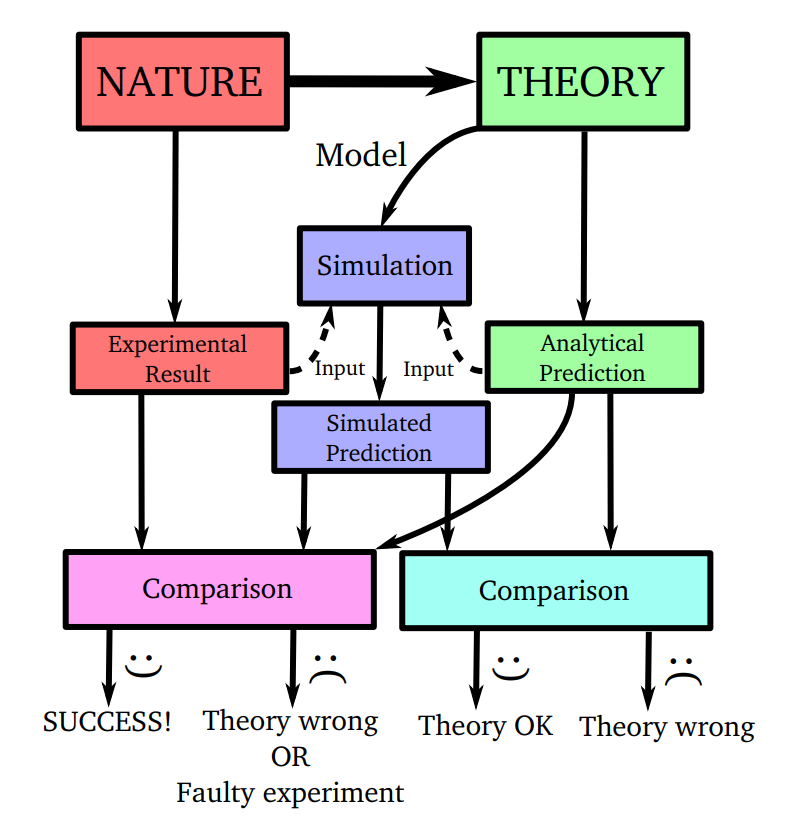
\includegraphics[width=0.8\linewidth]{fig/simulation-modeling-graph.png}
    \label{fig:sim_model_graph}
    \caption{แผนผังความเชื่อมโยงของระบบที่เราต้องศึกษา (Nature), ทฤษฎีหรือวิธีที่ใช้ในการศึกษา (Theory), แบบจำลองหรือโมเดล 
    (Model), ผลการทดลอง (Experimental Result), และผลการคำนวณหรือผลการทำนาย (Computational Results หรือ Prediction)}
\end{figure}

ภาพที่ \ref{fig:sim_model_graph} แสดงแผนผังเชื่อมโยงความแตกต่างระหว่าง Numerical Modeling กับ Computer Simulation 
นั้นก็คือใน Simulation นั้นระบบจำลองของเราจะถูกสร้างขึ้นมา เช่น เราสร้างระบบที่เป็นโมเลกุลน้ำหลาย ๆ โมเลกุลเกาะกลุ่มรวมกัน (Water 
Cluster) โดยเราหวังว่า Water Cluster ที่เราสร้างขึ้นมานี้จะสามารถเป็นตัวแทนของระบบของโมเลกุลน้ำจริง ๆ ได้ ซึ่งก็จะทำให้เราสามารถ%
ศึกษาคุณสมบัติต่าง ๆ ของโมเลกุลน้ำได้ตามต้องการ ส่วนการจำลองเชิงตัวหรือ Numerical Simulation นั้นจะเป็นการสร้างการทดลองเสมือนจริง 
(Virtual Experiments) ของระบบจำลองขึ้นมา อย่างไรก็ตามในบทความวิชาการทางด้านเคมีเชิงคำนวณหรือชีวเชิงคำนวณนั้นเรามักจะพบว่าคำว่า 
Modeling นั้นสามารถถูกแทนด้วยคำว่า Simulation ได้เช่นกัน

คำถามสำคัญที่หลายคนโดยเฉพาะอย่างนักวิทยาศาสตร์ที่ทำงานวิจัยเชิงการทดลองมักจะถามก็คือ \enquote{ทำไมการจำลองทางคอมพิวเตอร์ถึง%
มีความสำคัญ} คำตอบนั้นมีด้วยกันหลายข้อ ผู้เขียนขอสรุปเป็นประเด็นตามนี้ครับ

\begin{enumerate}
    \item การจำลองทางคอมพิวเตอร์นั้นเปรียบเสมือนเป็นสะพานเชื่อมโยงระหว่างทฤษฎีกับการทดลอง
    \item การทำการทดลองบางอย่างนั้นมีค่าใช้จ่ายที่สูงมากและมีความยากเพราะว่าตัวทฤษฎีนั้นซับซ้อนเกินไป ดังนั้นการจำลองทางคอมพิวเตอร์%
    นั้นจะเข้ามาช่วยในการจำลองการทดลองและทดสอบสมมติฐานเพื่อยืนยันทฤษฎีด้วย
    \item การจำลองทางคอมพิวเตอร์นั้นช่วยหาปัจจัยและเงื่อนไขที่เหมาะสมสำหรับการทดลองได้
    \item การจำลองทางคอมพิวเตอร์สามารถแสดงกระบวนการของระบบที่เราสนใจได้ ซึ่งอาจจะทำได้ยากในเชิงการทดลอง
    \item การจำลองทางคอมพิวเตอร์สามารถนำมาใช้ในการศึกษาปรากฏการณ์ที่การทดลองนั้นอาจจะให้ผลการทดลองที่ไม่ละเอียดพอ
\end{enumerate}

อย่างไรก็ตามผู้เขียนต้องขอสรุปเพิ่มเติมด้วยว่าการใช้แบบจำลองทางคอมพิวเตอร์เพียงอย่างเดียวนั้นจะเปล่าประโยชน์ถ้าหากว่าไม่มีผลการทดลองที่%
น่าเชื่อมายืนยันความถูกต้องของผลการคำนวณ ดังนั้นเคมีเชิงการทดลองกับเคมีเชิงคำนวณนั้นจึงเป็นศาสตร์ที่ต้องพึ่งพาอาศัยกัน

%----------------------------------------
\section{มาศึกษา Molecular Dynamics กันก่อน}
%----------------------------------------

ก่อนที่เราจะไปศึกษาวิธีการจำลองระบบโมเลกุลที่มีความซับซ้อนนั้นเราควรเริ่มต้นด้วยการศึกษาวิธีอย่างง่ายก่อนนั่นก็คือ Molecular Dynamics (MD) 
(จริง ๆ จะว่าไปแล้ววิธีนี้ก็ไม่ได้ง่ายนะครับ ถ้าลงรายละเอียดลึก ๆ แล้วก็มีความซับซ้อนมากพอสมควร ซึ่งในปัจจุบันนั้นก็มีการทำวิจัยที่เกี่ยวข้องกับ%
การพัฒนาเทคนิคของวิธี MD อย่างต่อเนื่อง) เราใช้เทคนิคการจำลองทางคอมพิวเตอร์ในการทำความเข้าใจคุณสมบัติของระบบที่ประกอบไปด้วยโมเลกุล 
ๆ โมเลกุลในเชิงโครงสร้างและอันตรกิริยาในระดับจุลภาคหรือหน่วยย่อย ซึ่งหน่วยย่อยในที่นี้ก็คือโมเลกุลนั่นเอง โดยเราสามารถแบ่งวิธีการจำลองออก%
ได้เป็น 2 วิธีคือ Molecular Dynamics (MD) กับ Monte Carlo (MC) และหนังสือเล่มนี้จะเน้นไปที่ MD ซึ่งเป็นวิธีที่สามารถนำมาใช้ในการศึกษา%
คุณสมบัติเชิงพลวัตได้ เช่น สัมประสิทธิ์การเคลื่อนที่ (Transport Coefficients), การตอบสนองต่อการรบกวนแบบที่ขึ้นกับเวลา (Time-dependt 
Response to Perturbation), และสเปกตรัม

ตัวอย่างของคุณสมบัติหรือปรากฏการณ์ที่เราสามารถใช้ MD เพื่อศึกษาได้นั้นมีดังต่อไปนี้

\noindent \textbf{เคมี (Chemistry)}

\begin{itemize}[topsep=0pt,noitemsep]
    \item Intra- and Intermolecular Interactions (Molecular Mechanics)
    \item Chemical Reactions
    \item Phase Transitions
    \item Free Energy Calculations
\end{itemize}

\noindent \textbf{วัสดุศาสตร์ (Materials Science)}

\begin{itemize}[topsep=0pt,noitemsep]
    \item Equilibrium Thermodynamics
    \item Phase Transitions
    \item Properties of Lattice Defects
    \item Nucleation and Surface Growth
    \item Heat/Pressure Processing
    \item Ion Implantation
    \item Properties of Nanostructures
\end{itemize}

\noindent \textbf{ชีวเชิงฟิสิกส์และชีวเคมี (Biophysics and Biochemistry)}

\begin{itemize}[topsep=0pt,noitemsep]
    \item Protein Folding
    \item Protein Structure Prediction
    \item Biocombatibility (Cell Wall Penetration, Chemical Processes)
    \item Molecular Docking
\end{itemize}

\noindent \textbf{การแพทย์ (Medicine)}

\begin{itemize}[topsep=0pt,noitemsep]
    \item Drug Design 
    \item Drug Discovery
\end{itemize}

%----------------------------------------
\section{ประวัติศาสตร์ของ Molecular Dynamics}
%----------------------------------------

\begin{itemize}
    \item 1953: Nicholas Metropolis และคณะได้ตีพิมพ์บทความวิจัยเรื่อง \enquote{Equation of State Calculations by Fast 
    Computing Machines}\autocite{metropolis1953} โดยบทความนี้เป็นเสมือนจุดเริ่มต้นของไอเดีย MD เลยก็ว่าได้ โดยเป็นครั้งแรกที่%
    ได้มีการประยุกต์ใช้เทคนิค Monte Carlo เพื่อแก้สมการที่อธิบายคุณสมบัติเชิงกายภาพของระบบที่ประกอบไปด้วยโมเลกุลที่มีอันตรกิริยาต่อกัน 
    โดยขั้นแรกคือสร้างเซตของตัวเลขสุ่ม (Random Number) เพื่อใช้เป็นตัวแทนของ Conformational Space แล้วก็ใช้ค่าของพลังงานเป็นตัว%
    ระบุความน่าจะเป็นของสถานะของระบบที่ศึกษา
    
    \item 1956: Berni J. Alder และ Thomas E. Wainwright ได้ตีพิมพ์บทความเรื่อง \enquote{Phase Transition for a Hard 
    Sphere System}\autocite{alder1957} ซึ่งถือได้ว่าเป็นงานวิจัยที่เป็นจุดเริ่มต้นของ MD เลยก็ว่าได้
    
    \item 1958: เป็นครั้งแรกที่นักวิทยาศาสตร์ค้นพบโครงสร้างสามมิติของโปรตีนได้โดยใช้เทคนิค X-ray โดยเผยแพร่ในบทความ 
    \enquote{A Three-Dimensional Model of the Myoglobin Molecule Obtained by X-Ray Analysis}\autocite{kendrew1958}

    \item 1964: บทความวิจัยเรื่อง \enquote{Correlations in the Motion of Atoms in Liquid Argon}\autocite{rahman1964} 
    โดย Aneesur Rahman ซึ่งเป็นผู้ที่ใช้ MD ในการคำนวณระบบของ Liquid Argon ซึ่งระบบที่ศึกษาตอนนั้นมี Argon ทั้งหมด 864 อะตอม 
    โดยคำนวณด้วยซุปเปอร์คอมพิวเตอร์  CDC 3600 โดยใช้ Lennard-Jones Potential นอกจากนี้ Aneesur Rahman ได้รับการยอบรับว่า%
    เป็นบิดาแห่งพลวัตเชิงโมเลกุลอีกด้วย (The Father of Molecular Dynamics)

    \item 1971: Aneesur Rahman และ Frank H. Stillinger ได้ตีพิมพ์บทความเรื่อง \enquote{Molecular Dynamics Study of 
    Liquid Water}\autocite{rahman1971} ซึ่งเป็นใช้ MD ในการจำลองระบบโมเลกุลน้ำที่มีจำนวนโมเลกุลคือ 216 โมเลกุล 

    \item 1975: Michael Levitt และ Arich Warshel ได้เผยแพร่บทความวิจัยเรื่อง \enquote{Computer Simulation of Protein 
    Folding}\autocite{levitt1975} ซึ่งเป็นครั้งแรกที่มีการนำเทคนิค MD มาใช้ในการจำลองการพับของโปรตีนโดยเป็นการศึกษาการพับของ 
    Bovine Pancreatic Trypsin Inhibitor (BPTI) จากโครงสร้างที่เป็นแบบสายเปิด

    \item 1979: David A. Case และ Martin Karplus ได้จำลองโปรตีนที่มีลิแกนด์เป็นโมเลกุลที่เข้าไปจับกับโปรแกรมด้วยเป็นครั้งแรก 
    โดยได้ตีพิมพ์งานวิจัยเรื่อง \enquote{Dynamics of ligand binding to heme protein}\autocite{case1979}

    \item 1980s: ในช่วงต้น ๆ ทศวรรษ 1980 นั้นเป็นช่วงที่มีการศึกษาชีวโมเลกุลด้วยการจำลอง MD เป็นจำนวนมาก รวมไปถึงมีการคำนวณ 
    Free Energy ด้วย

    \item 1985: Roberto Car Michele Parrinello ได้พัฒนาเทคนิค Car-Parrinello Molecular Dynamics (CPMD) ซึ่งเสนอใน%
    บทความเรื่อง \enquote{Unified Approach for Molecular Dynamics and Density-Functional Theory}\autocite{car1985} 
    โดยเป็นการนำเทคนิค Density Functional Theory มารวมกับ Born-Oppenheimer Molecular Dynamics

    \item 1988: Michael Levitt และ Ruth Sharon ได้คำนวณระบบของโปรตีนที่มีโมเลกุลน้ำเป็นตัวทำละลายและนำเสนอในบทความเรื่อง 
    \enquote{Accurate Simulation of Protein Dynamics in Solution}\autocite{levitt1988}

    \item 1990s: ในช่วงต้น ๆ ทศวรรษ 1990 นั้นก็ได้มีการพัฒนาศักย์ (Potential) ที่ใช้ในวิธี MD รวมถึงเทคนิคการเพิ่มประสิทธิภาพใน%
    การสุ่ม (Enhanced Sampling) อย่างต่อเนื่อง
\end{itemize}

%----------------------------------------
\section{อันตรกิริยาระหว่างโมเลกุล}
\idxboth{อันตรกิริยาระหว่างโมเลกุล}{Molecular Interactions}
%----------------------------------------

หัวใจสำคัญของ MD Simulations นั้นก็คืออันตรกิริยาระหว่างโมเลกุลนั่นก็คือ \enquote{แรง (Force)} โดยมีสมการสำคัญ 2 สมการที่ถือได้ว่า%
เป็นสมการหลักของ MD เลยก็ว่าได้ ดังนี้

\begin{equation}
    m_{i}\bm{\ddot{r}}_{i} = \bm{f}_{i}
\end{equation}

\begin{equation}
    \bm{f}_{i} = -\nabla_{i}V(\bm{r})
\end{equation}

\noindent สมการด้านบนนี้คือสมการการเคลื่อนที่ของนิวตัน (Newtonian Equation of Motion) สำหรับอะตอม $i$ โดยที่เป้าหมายของเรา%
นั้นก็คือการคำนวณแรง $\bm{f}$ ที่กระทำต่ออะตอมซึ่งสามารถคำนวณได้จากพลังงานศักย์ $V(\bm{r})$ นั่นเอง ส่วนเวกเตอร์ $\bm{r}$ นั้น%
ก็คือพิกัดคาร์ทีเซียนของตำแหน่งของอะตอม (นิวเคลียส) ทั้งหมดทุกอะตอมในโมเลกุลซึ่งเป็นพิกัดแบบ 3 มิติ

\begin{equation}
    \bm{r} = (\underbrace{r_{1,x}, r_{1,y}, r_{1,z}}_{\text{อะตอมตัวที่ 1}}, \dots, 
    \underbrace{r_{N,x}, r_{N,y}, r_{N,z}}_{\text{อะตอมตัวที่ $N$}})
\end{equation}

%----------------------------------------
\section{แบบฝึกหัด}
%----------------------------------------


